\documentclass[a4paper,11pt]{article}

\usepackage{graphicx}
\usepackage[english]{babel}
\usepackage{a4wide}
\usepackage{cite}               % will become: [2], [5]--[7]  (using cite.sty)
\usepackage{multirow}           % for multi-rows in tables
\usepackage{algorithm}
\usepackage{algorithmic}
\usepackage{amsmath}

\begin{document}

\title{Arithmetic Libraries User's Guide}
\author{Stefan Zwicky, Jeffrey St\"{a}hli, Christian Senning, Benjamin Weber}
\date{\today}
\maketitle

\section{Overview}
The arithmetic libraries are intended to make the VHDL-designer's life
easier. Basic arithmetic operations both on real and complex numbers
are provided as VHDL-functions together with the corresponding
bit-true \textsc{Matlab} functions.

The files under consideration are the following:
\begin{itemize}
\item \texttt{vhdl/VHDLTools/VHDLTools.vhd}
\item \texttt{vhdl/RealARITH/RealARITH.vhd}
\item \texttt{vhdl/ComplexARITH/ComplexARITH.vhd}
\item \texttt{matlab/VHDLTools/*.m}
\item \texttt{matlab/RealARITH/model/Real*.m}
\item \texttt{matlab/ComplexARITH/model/Complex*.m}
\end{itemize}
The package \texttt{VHDLTools.vhd} contains auxiliary functions such
as minimum(.), max(.) which are directly available in
\textsc{Matlab}. The functions of VHDLTools are used in
RealARITH. ComplexARITH is based on the RealARITH library.

The functions in Table~\ref{tab_arith_functions} are provided both in
\textsc{Matlab} and VHDL. There are some additional functions in the
\textsc{Matlab} directories, but they do not have a VHDL
counterpart. Table~\ref{tab_VHDL_functions} shows the functions that
are only provided in the VHDL library.

\begin{table}
  \centering
  \begin{tabular}{|l|l|c|l|c|}
    \hline
    Description & RealARITH & & ComplexARITH & \\
    \hline
    get word width (incl. sign bit(s)) & RealWIDTH & & ComplexWIDTH & \\
    % \hline
    merge imaginary and real part & - & & ComplexMERGE & \\
    % \hline
    changing the fixed-point representation & RealRESIZE & $\bullet$ &
    ComplexRESIZE & $\bullet$  \\
    % \hline
    absolute value & RealABS & $\bullet$ & - & \\
    % \hline
    negation & RealNEG & $\bullet$ &  ComplexNEG & $\bullet$ \\
    % \hline
    complex conjugate & - & & ComplexCONJ & $\bullet$ \\
    % \hline
    addition & RealADD & $\bullet$ & ComplexADD & $\bullet$ \\
    % \hline
    subtraction & RealSUB & $\bullet$ & ComplexSUB & $\bullet$ \\
    % \hline
    arithmetic shift left & RealASL & $\bullet$ & ComplexASL & $\bullet$ \\
    % \hline
    arithmetic shift right & RealASR & $\bullet$ &ComplexASR & $\bullet$ \\
    % \hline
    arithmetic shift (left or right) & RealAS & $\bullet$ & ComplexAS & $\bullet$ \\
    % \hline
    multiplication & RealMULT & $\bullet$ & ComplexMULT & $\bullet$ \\
    % \hline
    division & RealDIV & $\bullet$ & - & \\
    \hline
  \end{tabular}
  \caption{Arithmetic functions provided in VHDL as well as
    in \textsc{Matlab}. The dots indicate the support of data logging in \textsc{Matlab}} 
  \label{tab_arith_functions}
\end{table}

\begin{table}
  \centering
  \begin{tabular}{|l|l|}
    \hline
    get real part of signal & GetREAL \\
    \hline
    get imaginary part of signal & GetIMAG \\
    \hline
    multiply a complex number with a real one & ComplexRealMULT \\
    \hline
    division of a complex number by a real one & ComplexRealDIV \\
    \hline
  \end{tabular}
  \caption{Functions provided only in VHDL.} 
  \label{tab_VHDL_functions}
\end{table}


\section{Usage}

\subsection{Allowed Data Types}
The allowed data types in VHDL are unsigned and signed for the
RealARITH functions and signed for the ComplexARITH functions. An
exception is the shift argument in the arithmetic shift operations,
which must be of type unsigned for ASR and ASL and of type signed or a
constant integer for AS (shift left for positive values, shift right
for negative values).  In the RealARITH library, not all possible
combinations of signed and unsigned inputs/outputs are supported
(please refer to the VHDL package \texttt{RealARITH.vhd}).

\subsection{Fixed-point Representation}
The fixed-point word length is specified through a record constant of
type FixP in VHDL and a cell array in \textsc{Matlab} respectively.
It contains the following three items:
\begin{enumerate}
\item WIDTH\_INT is the number of bits for the integer part (excluding
  the sign bit)
\item WIDTH\_FRAC is the number of bits for the fractional part
\item SIG\_TYPE is either 'u' for unsigned signals or 's' for signed
  signals
\end{enumerate}
The SIG\_TYPE item is of type character in \textsc{Matlab} and of an
enumerated type (u,s) in VHDL. In \textsc{Matlab}, the three cell
array items must be defined always in the indicated order.

Even though it contradicts the definition, both WIDTH\_INT and
WIDTH\_FRAC can be negative. A negative value for WIDTH\_INT indicates
that the comma position is more to the ``left'' than the MSB of the
word, basically reducing WIDTH\_FRAC. However, the condition
\begin{equation*}
  \mathrm{WIDTH\_INT} + \mathrm{WIDTH\_FRAC} \geq 1
\end{equation*}
must always hold.
 
In VHDL, complex numbers are represented by real and imaginary part,
both having the same fixed-point representation. Real and imaginary
part are concatenated to a single signed value.
\begin{equation*}
  \texttt{Complex\_D(N downto 0) <= Imag\_D \& Real\_D;}
\end{equation*}
\texttt{Comple\_D} must always be of type signed.

In \textsc{Matlab}, complex numbers are represented by ``normal''
complex variables of type double. The fixed-point configuration is
contained in the value of the variable, by restricting it to the
maximal/minimal value according to WIDTH\_INT and by reducing its
accuracy according to WIDTH\_FRAC.

When changing the fixed-point representation of a value (either
directly with the resize function or through any other function that
calls the resize function), one must specify the behavior of the
circuit if the number of bits is not sufficient to represent that
value. There are two possibilities for both the most significant and
the least significant part of the word.
\begin{itemize}
\item Most significant bits:
  \begin{description}
    % \item{\bf Clp:} Clipping the most significant bits, running the
    %   risk of an overflow.
  \item{\bf Wrp:} Wraps the value if the value is out of
    range. (WARNING: The old argument {\bf Clp} should no longer be
    used)
  \item{\bf Sat:} Saturate to the largest/smallest representable value
    (or allowed value, refer to section~\ref{weird_number}).
  \end{description}
\item Least significant bits:
  \begin{description}
  \item{\bf Trc:} Truncate the least significant bits without
    considering their content.
  \item{\bf Rnd:} Round according to the content of the bits that are
    cut off.
  \end{description}
\end{itemize}

Combining these possibilities results in four quantization
possibilities:
\begin{equation*}
  \mathrm{QuantType} := \mathrm{(WrpTrc, WrpRnd, SatTrc, SatRnd)}
\end{equation*}

\subsection{Function Call}
In the following section, some examples of function calls are listed

\paragraph{VHDL} The fixed-point representation of signal A\_D is
denoted as A\_FixP or directly specified through e.g. (2,5,s).  The
first value in the brackets corresponds to WIDTH\_INT, the second to
WIDTH\_FRAC and the third to SIG\_TYPE. In VHDL, the FixP records of
both input and output must be provided as arguments.
\begin{itemize}
\item \texttt{Out\_D <=
    RealRESIZE(InA\_D,InA\_FixP,Out\_FixP,WrpTrc);}
\item \texttt{Out\_D <= ComplexRESIZE(InA\_D,(4,3,u),(3,2,u),WrpTrc);}
\end{itemize}
Functions with two input signals require the FixP constants for both
inputs and the output:
\begin{itemize}
\item \texttt{Out\_D <=
    RealADD(InA\_D,InB\_D,InA\_FixP,InB\_FixP,Out\_FixP,WrpRnd);}
\item \texttt{Out\_D <=
    ComplexMERGE(Real\_D,Imag\_D,Real\_FixP,Imag\_FixP,Out\_FixP,SatTrc);}
\end{itemize}
Exceptions are the arithmetic shift operations, where it is assumed
that the shift argument is integer (i.e. WIDTH\_INT is always 0).
\begin{itemize}
\item \texttt{Out\_D <=
    RealASL(InA\_D,Shift\_D,InA\_FixP,Out\_FixP,WrpRnd);}
\item \texttt{Out\_D <=
    ComplexAS(InA\_D,CONST,InA\_FixP,Out\_FixP,SatRnd);}
\end{itemize}
An additional argument is required for the complex multiplication. One
can choose between a fast architecture with four real-valued
multipliers and a slow architecture with only three real-valued
multipliers, but with an additional adder stage.
\begin{itemize}
\item \texttt{Out\_D <=
    ComplexMULT(InA\_D,InB\_D,InA\_FixP,InB\_FixP,Out\_FixP,WrpRnd,fast);}
\item \texttt{Out\_D <=
    ComplexMULT(InA\_D,InB\_D,InA\_FixP,InB\_FixP,Out\_FixP,WrpRnd,slow);}
\end{itemize}
Another extra argument is required for RealADDSUB. It selects between
addition ('0') and subtraction ('1').
\begin{itemize}
\item \texttt{Out\_D <=
    ComplexADDSUB(InA\_D,InB\_D,'1',(2,3,s),InB\_FixP,Out\_FixP,WrpTrc);}
\item \texttt{Out\_D <=
    ComplexADDSUB(InA\_D,InB\_D,'0',InA\_FixP,InB\_FixP,(5,8,s),WrpRnd);}
\end{itemize}
The functions GetREAL/GetIMAG and RealWIDTH/ComplexWIDTH are special
cases. They require only one input argument:
\begin{itemize}
\item \texttt{Real\_D <= GetREAL(Complex\_D); Imag\_D <=
    GetIMAG(Complex\_D);}
\item \texttt{WW\_REAL <= RealWIDTH(InA\_FixP); WW\_COMPLEX <=
    ComplexWIDTH(InB\_FixP);}
\end{itemize}
Additionally, there is a simplified version of ComplexMERGE. It
assumes that \texttt{Real\_D}, \texttt{Imag\_D} and \texttt{Out\_D}
all have the same FixP representation and just concatenates imaginary
and real part.
\begin{itemize}
\item \texttt{Out\_D <= ComplexMERGE(Real\_D,Imag\_D);}
\end{itemize}

\paragraph{MATLAB} Since the fixed-point representation of a
\textsc{Matlab} variable is inherently given by the accuracy of its
content, the corresponding \textsc{Matlab} functions require only the
FixP cell array of the return value.
\begin{itemize}
\item \texttt{Out = RealRESIZE(InA,\{-2,10,'s'\},'SatTrc');}
\item \texttt{Out = ComplexMULT(InA,InB,Out\_FixP,'WrpRnd');}
\end{itemize}
The only exception to this rule is the \texttt{RealDIV} function. It
can be called in two ways:
\begin{itemize}
\item \texttt{Out = RealDIV(inA,inB,FixP,QType);}
\item \texttt{Out =
    RealDIV(inA,inB,inA\_FixP,inB\_FixP,out\_FixP,QType);}
\end{itemize}
Only the latter call fully reflects the corresponding VHDL
implementation.

\subsection{The Weird Number} \label{weird_number} The most negative
number in a signed fixed-point configuration (i.e.  -1 for FixP =
(0,N)) is sometimes called the weird number because there is no
positive counterpart. In order to have a symmetric dynamic range, the
too small values are saturated to the next larger number which has a
positive counterpart (i.e. 11111 is saturated to 1001 instead of
1000). However, if the values are not saturated, it can happen
(intentionally or unintentionally) that the return value is exactly
the weird number.

\subsection{Data Logging in MATLAB}
The \texttt{RealRESIZE} function in \textsc{Matlab} is able to keep
track of specific data items. At the moment, it calculates the
complementary/inverse cumulative distribution function (ccdf/icdf) of
its input values.

\paragraph{Compilation:}
The \texttt{RealRESIZE} function supporting data logging in
\textsc{Matlab} is implemented as a \textsc{Mex} function written in
C. To compile this code for your machine, run \texttt{make} in the
\begin{itemize}
\item \texttt{asc\_matlab/Common/RealARITH/model/}
\end{itemize}
folder.

\paragraph{The \texttt{ArithLibStatistics} variable:}
To include the data logging ability in your simulations, you must
provide a global variable called \texttt{ArithLibStatistics} of type
\texttt{struct} at the beginning of our code. Every function
supporting data logging (see Table \ref{tab_arith_functions}) will
dynamically add a field to the \texttt{ArithLibStatistics} struct. The
\texttt{ArithLibStatistics} variable can be interpreted as a
one-dimensional array of structs. It is arranged as shown in Figure
\ref{fig.ArithLibStatistics}.
\begin{figure}[ht]
  \centering
  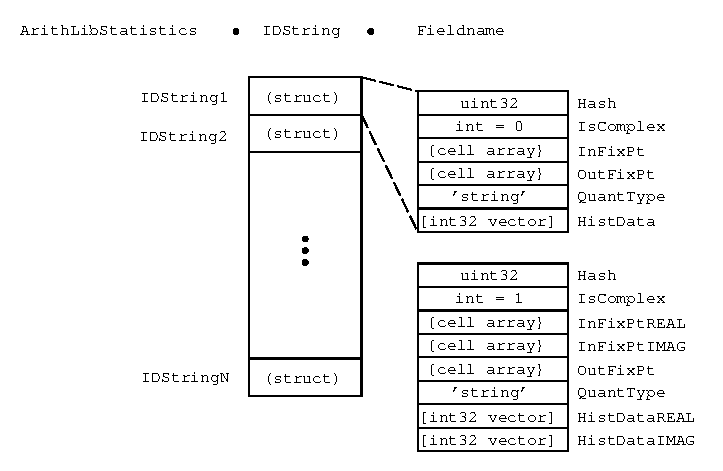
\includegraphics[width=0.8\textwidth]{ArithLibStatistics}
  \caption{The \texttt{ArithLibStatistics} variable (1-D array of
    structs). Note that the sub-structs are differently organized for
    real-valued and complex-valued arithmetic operations.}
  \label{fig.ArithLibStatistics}
\end{figure}

\paragraph{The Identifier String:}
In order to distinguish individual arithmetic operations, you need to
supply the functions with a unique identifier string. If you leave out
this string in the function call, \texttt{RealRESIZE} operates as
usual and will not log data from this particular function.  When a
function is called multiple times with the same identifier string, the
data is superimposed on the existing data.  Complex-valued operations
are internally split up into real and imaginary parts and the
identifier string is labeled accordingly by appending \texttt{(REAL)}
or \texttt{(IMAG)} to the given string.  The identifier string is
always the last argument in the function call.

\paragraph{Using the \texttt{ArithLibStatistics} variable:}
The data can be accessed using this scheme:
\begin{itemize}
\item \texttt{ArithLibStatistics.IDString} for a struct.
\item \texttt{ArithLibStatistics.IDString.FieldName} for the a
  specific field in the struct.
\end{itemize}
Refer to Figure \ref{fig.ArithLibStatistics} for valid fieldnames.

A function \texttt{generateHistPlots(m,n)} which creates
histogram-like plots of the complementary cumulative distribution
functions is provided. The arguments distribute the sub-plots in a
\texttt{m}$\times$\texttt{n} arrangement on the figure window. This
display function also creates new figures when the total number of
subplots exceeds the number \texttt{m}$\cdot$\texttt{n}.

A simple code example to illustrate the mentioned points is given
below.
\begin{verbatim}
% Global Log Variable
global ArithLibStatistics
ArithLibStatistics = struct; %initialize empty 1x1 struct

% Do some calc
Add01Out = RealADD(InA,InB,{4,2,'s'},'SatRnd','Add01');
...

% Graphical display
generateHistPlots(3,2); % (m,n) one figure holds m x n subplots
\end{verbatim}

\paragraph{The complementary cumulative distribution function plot:}
Figure \ref{fig.LoggerPlot} shows an example of such a plot. It
basically shows the ``total usage'' of the individual bits. One can
see, that the addition of two integer bits and one fractional bit to
the existing configuration at the output would give optimum results.
When overflows occur, a number designating the percentage of overflows
with respect to the total number of values is indicated for both
positive and negative input values.
\begin{figure}[ht]
  \centering
  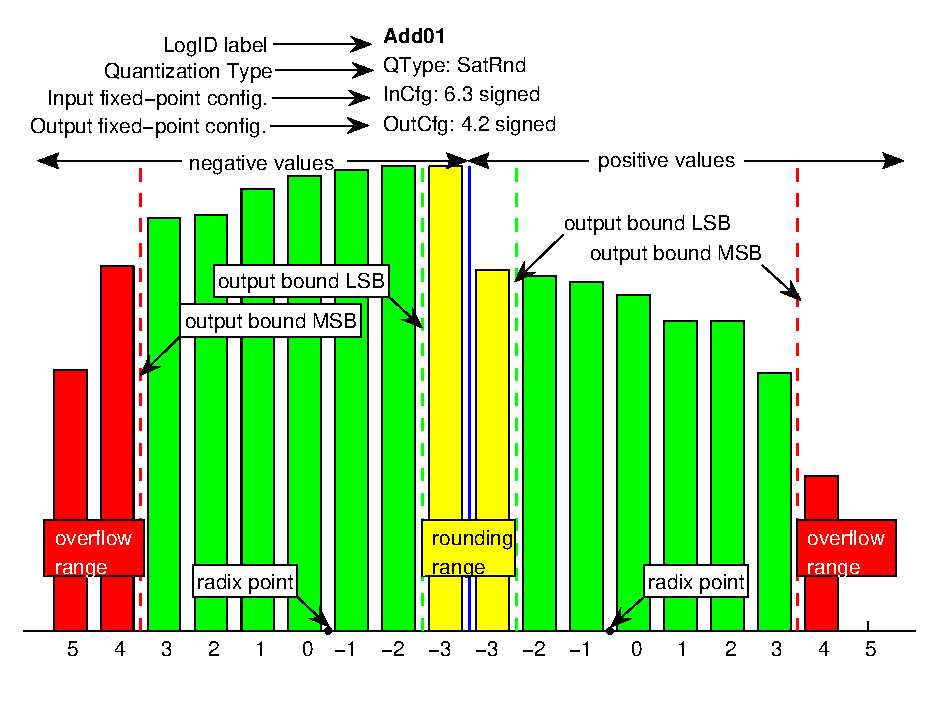
\includegraphics[width=0.6\textwidth]{LoggerPlotLabeled}
  \caption{Example of a plot. Positive numbers on the x-axis denote
    integer bits, negative ones label fractional bits.}
  \label{fig.LoggerPlot}
\end{figure}

\section{Outlook}
Features that might be added in the future:
\begin{itemize}
\item Defining a default value (e.g. WrpTrc) for QuantType. Replicate
  all functions without QuantType input.
\item Introducing a possibility to omit some FixP arguments
  (e.g. assume InA\_FixP = InB\_FixP = Oup\_FixP if only one FixP
  argument is provided)
\item Introducing a \texttt{ComplexDIV}.
\item Introducing a \texttt{ComplexANGLE} by means of a cordic.
\item Introducing a \texttt{ComplexABS} by means of a cordic.
\item \dots
\end{itemize}

\end{document}
